
\subsection{Traditional Distance Metrics}

The testing results of the simple distance metrics above are shown in Table \ref{tab:simple}. We can see that among three Minkowski distances, Euclidean distance gets an accuracy one percent higher than Manhattan. However, Chebyshev distance perfroms much worse than them for a gap around 10\%. Cosine distance also performs well for an accuracy above 90\%, and we also note that the classifier using Cosine distance 
computes fastest in these metrics.

\begin{table}[htbp]
    \centering
    \caption{Accuracy of KNN with Simple Distance Metrics}
    \begin{tabular}{@{}ccccc@{}}
    \toprule
    $K$     &   Manhattan   &   Euclidean   &   Chebyshev   &   Cosine  \\ \midrule
    3       &   88.18\%     &   88.83\%     &   77.69\%     &  89.85\%  \\
    4       &   88.04\%     &   88.89\%     &   78.30\%     &   89.80\% \\
    5       &   \textbf{88.50\%} &   89.27\%&   78.61\%     &   90.37\% \\
    6       &   88.33\%     &   89.33\%     &   78.81\%     &   90.13\% \\
    7       &   88.48\%     &   \textbf{89.45\%} &   \textbf{79.17\%}   &   \textbf{90.53\%}   \\ 
    8       &   88.09\%     &   89.10\%     &   78.83\%     &   90.43\% \\
    9       &   88.30\%     &   89.18\%     &   79.14\%     &   90.41\% \\
    10      &   88.06\%     &   89.16\%     &   78.91\%     &   90.44\% \\
    15      &   87.58\%     &   88.89\%     &   78.48\%     &   90.37\% \\
    20      &   87.05\%     &   88.68\%     &   78.03\%     &   90.17\% \\\bottomrule
    \end{tabular}
    \label{tab:simple}
\end{table}



\subsection{Supervised Metric Learning}


\subsubsection{LMNN: Large Margin Nearest Neighbor Metric Learning}
% todo
In this section, there are two "k" values which has a big influence on experiment result. The first one matters in LMNN metric learning process, denoted as $K_1$,  and the other one is used in KNN classifying process, denoted as $K_2$. we take different $K_1$ and $K_2$ on this experiment and get the result in table \ref{tab:lmnn_k}.
\begin{table}[htbp]
\centering
\caption{KNN Accuracy of LMNN with K neighbors}
\scriptsize
\begin{tabular}{@{}cccccccccccc@{}}
\toprule
$K_1 \backslash K_2$ & 3 & 4 & 5 & 6 & 7 & 8 & 9 & 10 & 15 & 20 \\ \midrule
3 & 90.77\% & 91.04\% & 91.41\% & 91.44\% & 91.51\% & 91.42\% & 91.75\% & 91.69\% & 91.60\% & 91.28\% \\
7 & 91.84\% & 91.98\% & 92.18\% & 92.36\% & 92.44\% & 92.26\% & 92.37\% & 92.40\% & 92.18\% & 92.15\% \\
10 & 91.83\% & 92.12\% & 92.26\% & 92.36\% & 92.58\% & 92.58\% & 92.63\% & 92.54\% & 92.52\% & 92.42\% \\
15 & 92.20\% & 92.39\% & 92.68\% & 92.48\% & 92.58\% & 92.63\% & 92.74\% & 92.71\% & 92.71\% & 92.62\% \\
20 & 92.52\% & 92.32\% & 92.73\% & 92.62\% & 92.89\% & 92.68\% & 92.85\% & 92.79\% & 92.80\% & 92.79\% \\
30 & 90.38\% & 90.75\% & 91.39\% & 91.23\% & 91.55\% & 91.56\% & 91.58\% & 91.65\% & 91.75\% & 91.83\% \\
\bottomrule
\end{tabular}
\label{tab:lmnn_k}
\end{table}

We can the accuracy trend in fig\ref{fig:lmnn_k}. As is shown, when $K_1$ takes the value 20, KNN has a relatively good classification performance as a whole. This is related to the distribution of samples. When K1 is too small, it is not enough to learn a suitable projection with the help of neighbors; While when K1 is too large, it is easy to introduce disturbing neighbor samples.
\begin{figure}
\centering
\begin{minipage}[t]{0.48\linewidth}
\centering
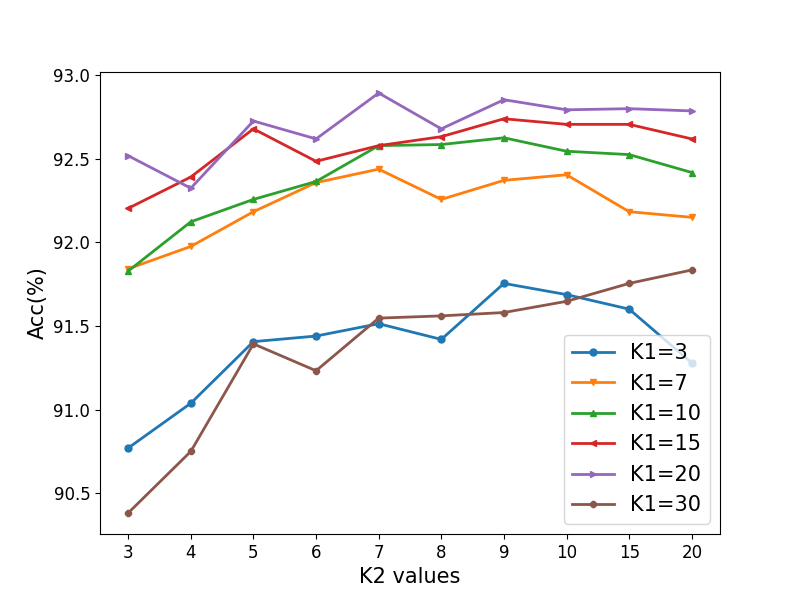
\includegraphics[width=1.0\linewidth]{img/LMNN_K.png}
\caption{The Influence of K values on Result}
\label{fig:lmnn_k}
\end{minipage}
\begin{minipage}[t]{0.48\linewidth}
\centering
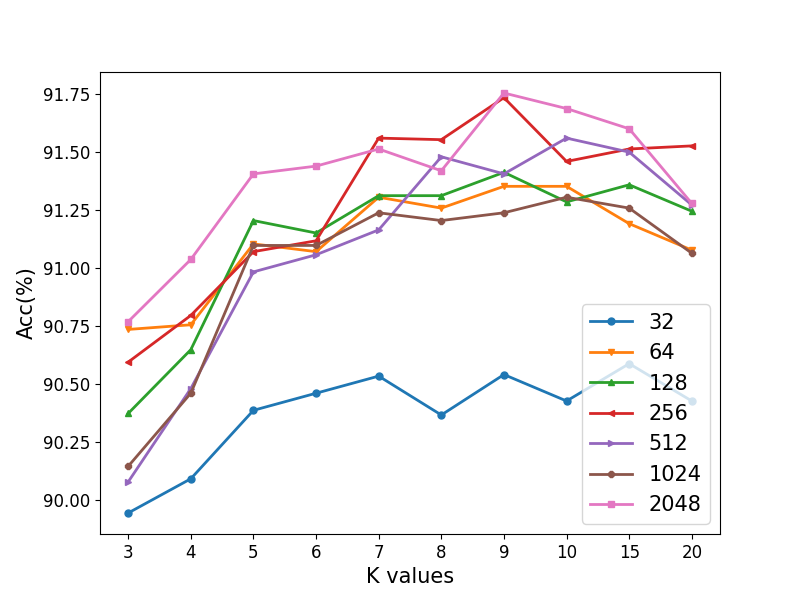
\includegraphics[width=1.0\linewidth]{img/LMNN_res.png}
\caption{The Influence of Feature Dimensions on Result}
\label{fig:lmnn_res}
\end{minipage}
\end{figure}


We also selected different degrees of dimensionality reduction to observe the influence of feature dimensions on the final classification. We show the result and trend in table \ref{tab:lmnn} and fig \ref{fig:lmnn_res}. For LMNN algorithm, The best classification effect is achieved by retaining the original features. However, with the increase of K parameter in KNN, it shows a downward trend. In general, when K is small, it is better to keep the higher dimension, and when K is large, reducing the dimension to 256 achieves a better result.


\begin{table}[htbp]
\centering
\caption{KNN Accuracy of LMNN with Different Features}
\begin{tabular}{@{}cccccccc@{}}
\toprule
$K_2 \backslash $Features & 32 & 64 & 128 & 256 & 512 & 1024 & 2048 \\ \midrule
3 & 89.946\% & 90.736\% & 90.374\% & 90.595\% & 90.080\% & 90.147\% & 90.770\% \\
4 & 90.093\% & 90.756\% & 90.649\% & 90.796\% & 90.482\% & 90.462\% & 91.038\% \\
5 & 90.388\% & 91.105\% & 91.205\% & 91.071\% & 90.984\% & 91.098\% & 91.406\% \\
6 & 90.462\% & 91.071\% & 91.151\% & 91.118\% & 91.058\% & 91.098\% & 91.439\% \\
7 & 90.535\% & 91.306\% & 91.312\% & 91.560\% & 91.165\% & 91.239\% & 91.513\% \\
8 & 90.368\% & 91.259\% & 91.312\% & 91.553\% & 91.480\% & 91.205\% & 91.419\% \\
9 & 90.542\% & \textbf{91.352\%} & \textbf{91.413\%} & \textbf{91.734\%} & 91.406\% & 91.239\% & \textbf{91.754\%} \\
10 & 90.428\% & 91.352\% & 91.285\% & 91.460\% & \textbf{91.560\%} & \textbf{91.306\%} & 91.687\% \\
15 & \textbf{90.589\%} & 91.192\% & 91.359\% & 91.513\% & 91.500\% & 91.259\% & 91.6\% \\
20 & 90.428\% & 91.078\% & 91.245\% & 91.527\% & 91.272\% & 91.064\% & 91.279\% \\
\bottomrule
\end{tabular}
\label{tab:lmnn}
\end{table}


\subsubsection{NCA: Neighborhood Component Analysis}
        % to do
        For NCA algorithm, the two parameters that have influence on the result comparison are sample feature dimension and the number of neighbors in KNN cluster. We take different values on these two variables and get the result in table \ref{tab:nca}.
\begin{table}[htbp]
    \centering
    \caption{KNN Accuracy of NCA with Different Features}
    \begin{tabular}{@{}cccccccc@{}}
    \toprule
    $K \backslash $Features & 32 & 64 & 128 & 256 & 512 & 1024 & 2048 \\ \midrule
    3 & 90.019\% & 88.827\% & 88.841\% & 88.753\% & 88.566\% & 88.211\% & 87.943\% \\
    4 & 90.180\% & 88.854\% & 89.242\% & 88.887\% & 88.586\% & 88.191\% & 88.057\% \\
    5 & 90.622\% & 89.410\% & 89.611\% & 89.175\% & 88.995\% & 88.392\% & 88.432\% \\
    6 & 90.488\% & 89.229\% & 89.631\% & 89.336\% & 89.088\% & 88.512\% & 88.224\% \\
    7 & 90.703\% & 89.604\% & 89.671\% & \textbf{89.638\%} & \textbf{89.343\%} & \textbf{88.948\%} & 88.519\% \\
    8 & 90.716\% & 89.490\% & 89.731\% & 89.551\% & 89.169\% & 88.566\% & 88.385\% \\
    9 & 90.823\% & \textbf{89.658\%} & 89.651\% & 89.417\% & 89.276\% & 88.82\% & \textbf{88.546\%} \\
    10 & 90.723\% & 89.497\% & \textbf{89.792\%} & 89.396\% & 89.095\% & 88.606\% & 88.432\% \\
    15 & 90.850\% & 89.504\% & 89.671\% & 89.283\% & 88.834\% & 88.184\% & 88.110\% \\
    20 & \textbf{90.897\%} & 89.142\% & 89.363\% & 88.794\% & 88.432\% & 87.796\% & 87.675\% \\ \bottomrule
    \end{tabular}
    \label{tab:nca}
\end{table}

    We look at the results in a line chart \ref{fig:nca_res}. The K value for maximum accuracy varies with the selection of feature dimensions, but the overall range is between 7 and 10. This indicates that when a dimension that can fully distinguish features is maintained, a moderate range of K values can be selected to achieve better results. 
    
    In addition, the dimension reduction to 32-dimensional features in this experiment can achieve a surprising accuracy, which is confused. We believe that this simplified feature is more conducive to NCA learning better projection methods in the neighborhood.
    \begin{figure}[htbp]
        \centering
        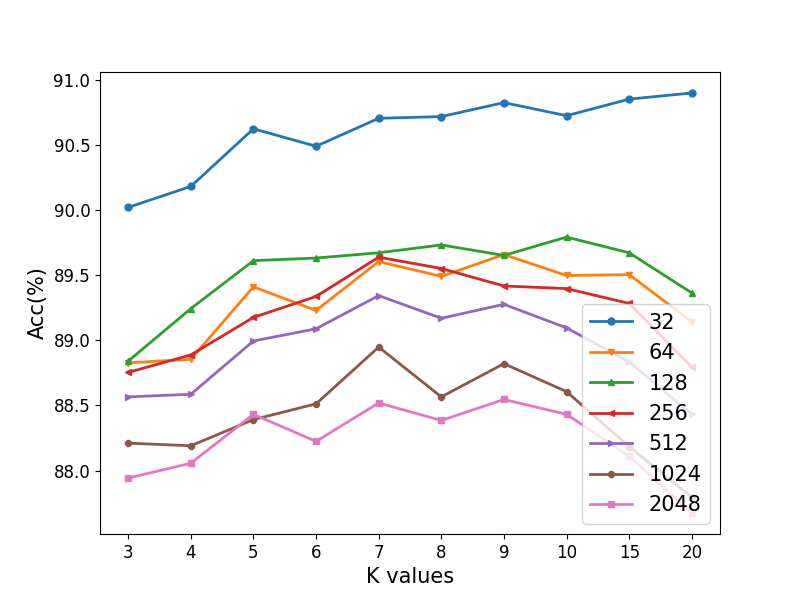
\includegraphics[width=0.6\linewidth]{img/NCA_res.png}
        \caption{The Result of NCA}
        \label{fig:nca_res}
    \end{figure}



\subsubsection{LFDA: Local Fisher Discriminant Analysis}
        Similar to LMNN method, $K_1$ and $K_2$ were selected here for the first experiment, and K2 and characteristic dimension, were selected for the second experiment. We show the result in table \ref{tab:lfda_k} and \ref{tab:lfda}.
        
        From the result we can see that when $K_1$ equals to 20, The performance is optimal overall. One thing to notice is that when $K_1$ takes 3 and 7, there is no any effect on the results. This has to do with the distribution of sample features, when we take different K value on a small scale, neighbors of the sample did not change the LFDA results. And there is also a trend that when we increase $K_2$ in a range greater than 7, the overall performance of KNN classification shows decline.
        
         Another factor is feature dimension. We can find that when the number of features is a moderate value such as 64, 128, 256, KNN classification can achieve the best results which is different from LMNN methods.
        
\begin{table}[htbp]
    \centering
    \caption{KNN Accuracy of LFDA with K neighbors}
    \scriptsize
    \begin{tabular}{@{}cccccccccccc@{}}
    \toprule
    $K_1 \backslash K_2$ & 3 & 4 & 5 & 6 & 7 & 8 & 9 & 10 & 15 & 20 \\ \midrule
    3 & 86.33\% & 86.18\% & 86.68\% & 86.34\% & 86.5\% & 86.32\% & 86.3\% & 86.21\% & 85.92\% & 85.52\% \\
    7 & 86.33\% & 86.18\% & 86.68\% & 86.34\% & 86.5\% & 86.32\% & 86.3\% & 86.21\% & 85.92\% & 85.52\% \\
    10 & 86.04\% & 85.82\% & 86.05\% & 85.77\% & 86.01\% & 85.79\% & 85.81\% & 85.69\% & 85.52\% & 85.04\% \\
    15 & 86.17\% & 86.21\% & 86.53\% & 86.46\% & 86.37\% & 86.42\% & 86.44\% & 86.25\% & 86.09\% & 85.74\% \\
    20 & 86.96\% & 86.82\% & 87.01\% & 86.94\% & 86.94\% & 86.75\% & 86.87\% & 86.72\% & 86.56\% & 86.31\% \\
    30 & 85.51\% & 85.42\% & 85.61\% & 85.52\% & 85.59\% & 85.32\% & 85.48\% & 85.22\% & 85.1\% & 84.53\% \\
    \bottomrule
    \end{tabular}
    \label{tab:lfda_k}
\end{table}
    \begin{figure}
        \centering
        \begin{minipage}[t]{0.48\linewidth}
            \centering
            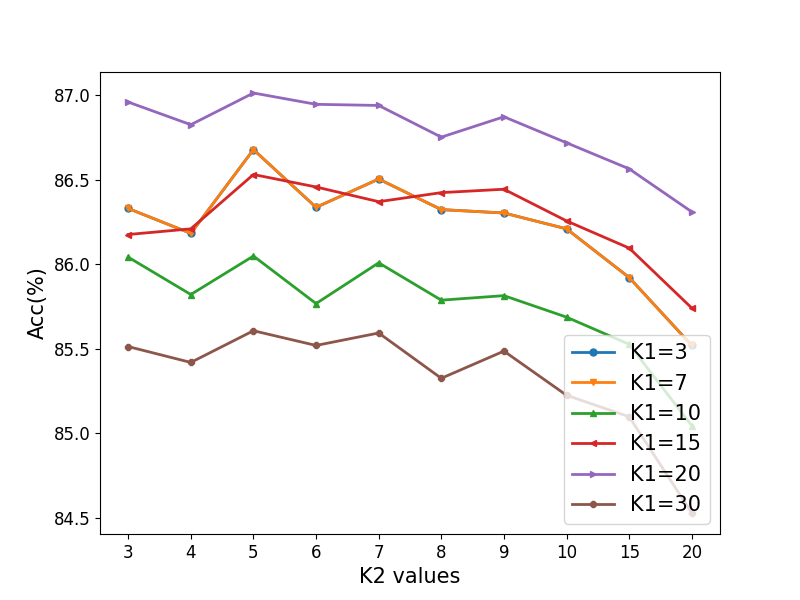
\includegraphics[width=1.0\linewidth]{img/LFDA_K.png}
            \caption{The Influence of K values on Result}
            \label{fig:lfda_k}
        \end{minipage}
        \begin{minipage}[t]{0.48\linewidth}
            \centering
            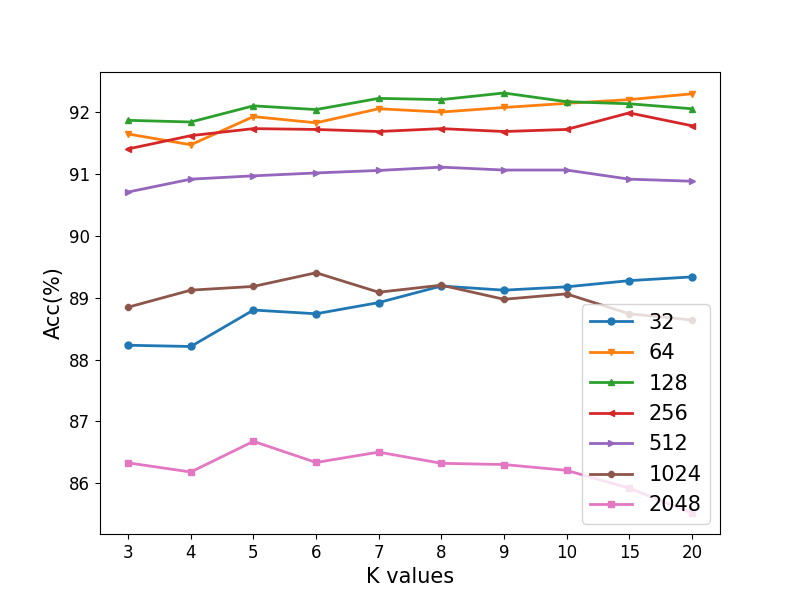
\includegraphics[width=1.0\linewidth]{img/LFDA_res.png}
            \caption{The Influence of Feature Dimensions on Result}
            \label{fig:lfda_res}
        \end{minipage}
    \end{figure}
    
\begin{table}[htbp]
    \centering
    \caption{KNN Accuracy of LFDA with Different Features}
    \begin{tabular}{@{}cccccccc@{}}
    \toprule
    $K_2 \backslash $Features & 32 & 64 & 128 & 256 & 512 & 1024 & 2048 \\ \midrule
    3 & 88.231\% & 91.647\% & 91.868\% & 91.406\% & 90.709\% & 88.847\% & 86.329\% \\
    4 & 88.211\% & 91.473\% & 91.841\% & 91.620\% & 90.917\% & 89.122\% & 86.181\% \\
    5 & 88.800\% & 91.928\% & 92.103\% & 91.734\% & 90.971\% & 89.182\% & \textbf{86.677\%} \\
    6 & 88.740\% & 91.828\% & 92.042\% & 91.721\% & 91.017\% & \textbf{89.403\%} & 86.335\% \\
    7 & 88.921\% & 92.056\% & 92.223\% & 91.687\% & 91.058\% & 89.088\% & 86.503\% \\
    8 & 89.189\% & 92.002\% & 92.203\% & 91.734\% & \textbf{91.111\%} & 89.202\% & 86.322\% \\
    9 & 89.122\% & 92.076\% & \textbf{92.310\%} & 91.687\% & 91.064\% & 88.974\% & 86.302\% \\
    10 & 89.175\% & 92.143\% & 92.170\% & 91.721\% & 91.064\% & 89.062\% & 86.208\% \\
    15 & 89.276\% & 92.203\% & 92.136\% & \textbf{91.989\%} & 90.917\% & 88.740\% & 85.920\% \\
    20 & \textbf{89.336\%} & \textbf{92.297\%} & 92.056\% & 91.781\% & 90.884\% & 88.640\% & 85.518\% \\
    \bottomrule
    \end{tabular}
    \label{tab:lfda}
\end{table}
    


\subsubsection{MLKR: Metric Learning for Kernel Regression}
        In this section, we mainly verify the parameter of feature numbers. The result is shown in table \ref{tab:mlkr}.  We can see in fig \ref{fig:mlkr_res}, most curves follow the same trend. Moderate dimensionality reduction leads to better performance, which is similar to the choice of K value. Obviously, the appropriate dimension can make the sample projected by the kernel function into a space that is easier to classify. Similarly, a moderate K value can also maintain the distance characteristic from the neighbors while avoiding the interference of other samples. These two factors contribute to the results in the figure and table.

\begin{table}[htbp]
    \centering
    \caption{KNN Accuracy of MLKR with Different Features}
    \begin{tabular}{@{}cccccccc@{}}
    \toprule
    $K \backslash $Features & 32 & 64 & 128 & 256 & 512 & 1024 & 2048 \\ \midrule
    3 & 86.844\% & 88.66\% & 88.914\% & 88.707\% & 88.285\% & 88.010\% & 87.621\% \\
    4 & 86.931\% & 88.733\% & 89.196\% & 88.660\% & 88.305\% & 88.084\% & 87.635\% \\
    5 & 87.374\% & 89.236\% & 89.571\% & 89.162\% & 88.854\% & 88.472\% & 88.050\% \\
    6 & 87.300\% & 89.182\% & 89.443\% & 89.068\% & 88.914\% & 88.271\% & 87.749\% \\
    7 & 87.662\% & 89.517\% & \textbf{89.745\%} & 89.484\% & 89.075\% & 88.472\% & 88.003\% \\
    8 & 87.983\% & 89.403\% & 89.685\% & 89.490\% & \textbf{89.115\%} & 88.358\% & 87.943\% \\
    9 & \textbf{88.017\%} & \textbf{89.571\%} & 89.705\% & \textbf{89.537\%} & 89.068\% & \textbf{88.559\%} & 87.930\% \\
    10 & 87.856\% & 89.504\% & 89.658\% & 89.457\% & 88.847\% & 88.385\% & \textbf{88.070\%} \\
    15 & 87.923\% & 89.463\% & 89.430\% & 89.303\% & 88.566\% & 88.070\% & 87.615\% \\
    20 & 87.581\% & 89.075\% & 89.135\% & 88.787\% & 88.137\% & 87.608\% & 87.059\% \\
    \bottomrule
    \end{tabular}
    \label{tab:mlkr}
\end{table}

    \begin{figure}[htbp]
        \centering
        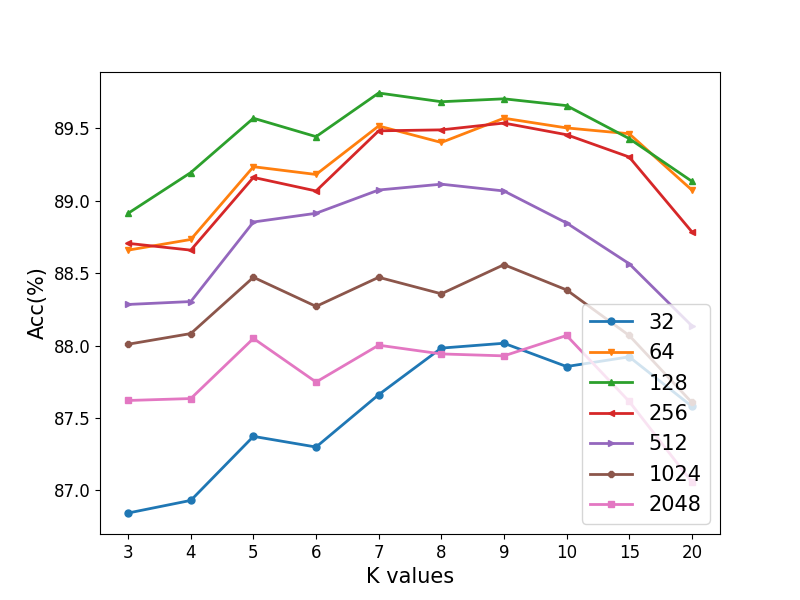
\includegraphics[width=0.6\linewidth]{img/MLKR_res.png}
        \caption{The Result of MLKR}
        \label{fig:mlkr_res}
    \end{figure}


\subsection{Weakly Supervised Metric Learning}

\subsubsection{ITML: Information Theoretic Metric Learning}

It is impossible to sample too many number of samples because the  memory for computation is limited.  So the method requires an additional parameter \texttt{num\_constraints}, which indicates that the method will try to build \texttt{num\_constraints} positive pairs and \texttt{num\_constraints} negative pairs. We take different \texttt{num\_constraints} and try to perform classification on the same train-test split of data-set with respect to different $K$ neighbors, to see how the model performs under different scale of pair sampling. The result of experiments on ITML is demonstrated in Table \ref{tab:itml}.

\begin{table}[h]
\centering
\caption{KNN Accuracy of ITML with different sample numbers \label{tab:itml}}
\begin{tabular}{cccccc}
\hline
K   & 50       & 100      & 200      & 500      & 1000     \\ \hline
3   & 88.177\% & 87.367\% & 86.208\% & \textbf{82.812}\% & \textbf{79.597}\% \\
4   & 88.043\% & 86.871\% & 85.887\% & 82.202\% & 79.168\% \\
5   & 88.599\% & \textbf{87.601}\% & \textbf{86.322}\% & 82.618\% & 79.463\% \\
6   & 88.573\% & 87.159\% & 86.034\% & 82.142\% & 79.074\% \\
7   & \textbf{88.640}\% & 87.367\% & 86.154\% & 82.196\% & 78.900\% \\
8   & 88.506\% & 87.240\% & 85.887\% & 82.042\% & 78.545\% \\
9   & 88.566\% & 87.340\% & 85.967\% & 82.042\% & 78.525\% \\
10  & 88.291\% & 87.119\% & 85.592\% & 81.747\% & 78.163\% \\
15  & 87.809\% & 86.911\% & 85.478\% & 80.883\% & 77.507\% \\
20  & 87.487\% & 86.376\% & 85.036\% & 80.293\% & 76.790\% \\
30  & 86.838\% & 85.451\% & 84.199\% & 79.081\% & 75.484\% \\ \hline
Avg & \textbf{88.139\%} & 86.982\% & 85.706\% & 81.642\% & 78.292\% \\ \hline
\end{tabular}
\end{table}

It can be seen that fewer samples and a relatively small K leads to better performance on ITML metric.

Note that 50 samples are only a very small fraction of the whole data-set, and that larger sample numbers result in a cascade in the classification accuracy, indicating that the metrics we learned from ITML will not help improve the classification performance. We wonder if there exists an improved metric learning solution based on ITML. It turned out that preprocessing the data-set with \emph{PCA} can help ITML exert its true power.

We perform PCA on the original data-set and reduce every data point from 2048 dimensions to 64 dimensions. The KNN accuracy with ITML learned metrics is listed in Table \ref{tab:itml2}.

\begin{table}[h]
\centering
\caption{KNN Accuracy on PCA reduced data-set of ITML with different sample numbers \label{tab:itml2}}
\footnotesize
\begin{tabular}{ccccccccc}
\hline
K   & 50       & 100      & 200      & 500      & 1000     & 5000     & 10000    & 20000    \\ \hline
3   & 87.360\% & 87.528\% & 88.465\% & 88.887\% & 89.276\% & 89.175\% & 89.229\% & 89.249\% \\
4   & 87.220\% & 87.561\% & 88.445\% & 89.008\% & 89.162\% & 89.236\% & 89.323\% & 89.524\% \\
5   & 87.682\% & 87.943\% & 89.041\% & 89.624\% & 89.805\% & 89.778\% & 89.912\% & 89.865\% \\
6   & 87.688\% & 88.090\% & 89.102\% & 89.624\% & 89.685\% & 89.718\% & 89.651\% & 90.107\% \\
7   & 87.943\% & \textbf{88.305\%} & \textbf{89.457\%} & 89.510\% & \textbf{89.872\%} & 89.939\% & \textbf{90.113\%} & 90.073\% \\
8   & 87.923\% & 88.204\% & 89.129\% & 89.571\% & 89.798\% & 89.993\% & 89.966\% & \textbf{90.274\%} \\
9   & \textbf{87.990\%} & 88.110\% & 89.296\% & 89.751\% & 89.785\% & 90.013\% & 90.086\% & 90.261\% \\
10  & 87.909\% & 88.177\% & 89.269\% & \textbf{89.812\%} & 89.678\% & \textbf{90.127\%} & 90.073\% & 90.173\% \\
15  & 87.595\% & 87.856\% & 89.055\% & 89.772\% & 89.772\% & 90.026\% & 90.033\% & 90.167\% \\
20  & 87.534\% & 87.494\% & 88.928\% & 89.597\% & 89.577\% & 89.952\% & 89.973\% & 90.026\% \\
30  & 87.012\% & 86.885\% & 88.305\% & 89.209\% & 89.082\% & 89.584\% & 89.651\% & 89.671\% \\ \hline
Avg & 87.623\% & 87.832\% & 88.954\% & 89.488\% & 89.590\% & 89.776\% & 89.819\% & \textbf{89.945}\% \\ \hline
\end{tabular}
\end{table}

After PCA, The training accuracy grows monotonously as we increase the sampling number, indicating that the ITML metric learning distance can indeed boost the classification performance. We conclude that the accuracy of ITML metrics on PCA-reduced data-set can outperform the euclidean metrics with sufficient sampling.

\begin{figure}
    \centering
    \begin{minipage}[t]{0.48\linewidth}
        \centering
        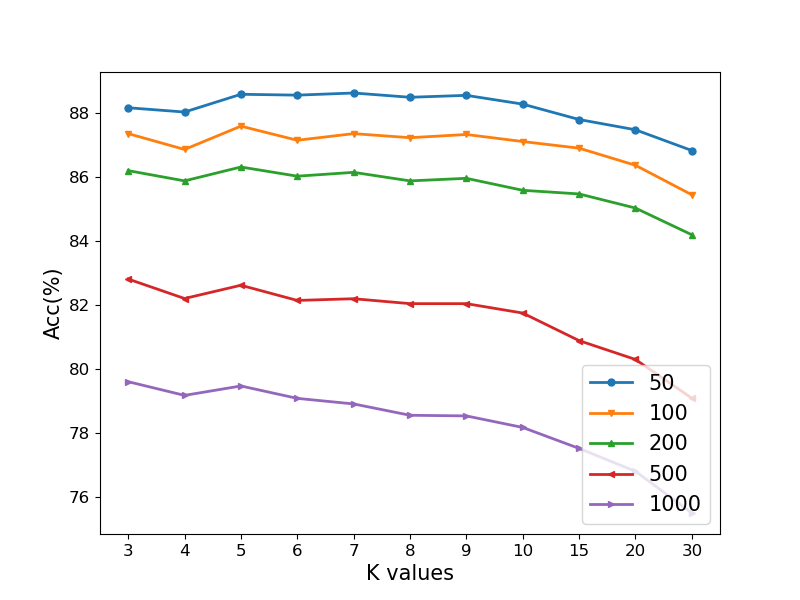
\includegraphics[width=1.0\linewidth]{img/ITML-k.png}
        \caption{Accuracy of ITML metric learning}
        \label{fig:itml}
    \end{minipage}
    \begin{minipage}[t]{0.48\linewidth}
        \centering
        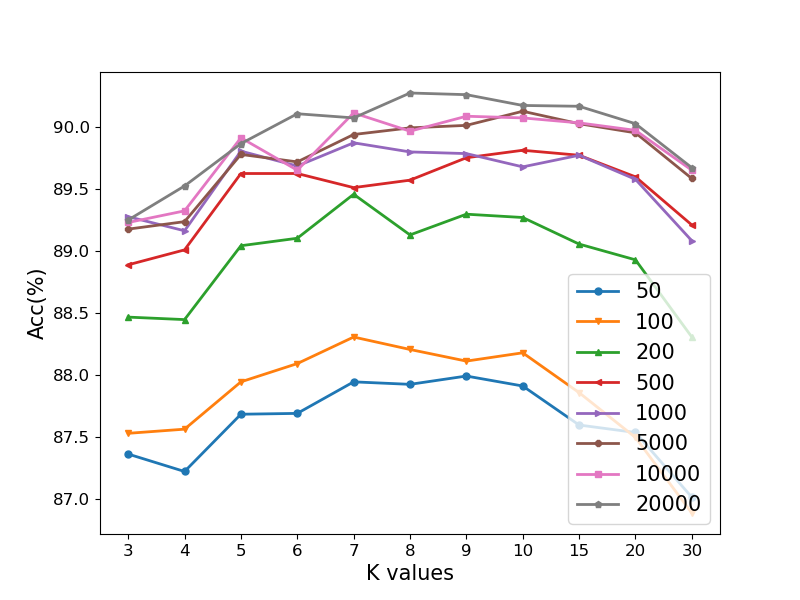
\includegraphics[width=1.0\linewidth]{img/ITML-PCA-k.png}
        \caption{Accuracy of ITML after PCA}
        \label{fig:itml-pca}
    \end{minipage}
\end{figure}


\subsubsection{LSML: Least Squared-residual Metric Learning}

We take different \texttt{num\_constraints} and try to perform classification on the same train-test split of data-set with respect to different $K$ neighbors. The result of experiments on LSML is demonstrated in Table \ref{tab:lsml}.

\begin{table}[h]
\centering
\caption{KNN Accuracy of LSML with different sample numbers \label{tab:lsml}}
\begin{tabular}{cccccc}
\hline
K   & 50       & 100      & 200      & 500      & 1000     \\ \hline
3   & 88.834\% & 88.894\% & 88.834\% & 89.062\% & 89.088\% \\
4   & 88.921\% & 88.834\% & 88.995\% & 89.149\% & 89.169\% \\
5   & 89.289\% & 89.242\% & 89.370\% & 89.544\% & 89.396\% \\
6   & 89.229\% & 89.242\% & 89.396\% & 89.484\% & 89.396\% \\
7   & \textbf{89.390\%} & \textbf{89.430\%} & \textbf{89.423\%} & \textbf{89.591\%} & \textbf{89.524\%} \\
8   & 89.236\% & 89.155\% & 89.196\% & 89.410\% & 89.350\% \\
9   & 89.303\% & 89.329\% & 89.296\% & 89.463\% & 89.490\% \\
10  & 89.196\% & 89.068\% & 89.175\% & 89.423\% & 89.269\% \\
15  & 88.961\% & 88.961\% & 89.008\% & 89.075\% & 88.901\% \\
20  & 88.686\% & 88.619\% & 88.546\% & 88.767\% & 88.539\% \\
30  & 87.923\% & 87.970\% & 87.775\% & 88.050\% & 87.722\% \\ \hline
Avg & 88.997\% & 88.977\% & 89.001\% & \textbf{89.183}\% & 89.077\% \\ \hline
\end{tabular}
\end{table}

It can be seen that the number of samples makes minor difference to the classification accuracy and that a moderate K is preferred for LSML metric learning.

\begin{table}[h]
\centering
\caption{KNN Accuracy of LSML on PCA-reduced data-set with different sample numbers \label{tab:lsml2}}
\begin{tabular}{cccccccc}
\hline
    & 200      & 500      & 1000     & 2000     & 5000     & 10000    & 20000    \\ \hline
3   & 89.289\% & 89.544\% & 89.356\% & 89.396\% & 89.417\% & 89.403\% & 89.490\% \\
4   & 89.504\% & 89.551\% & 89.631\% & 89.551\% & 89.624\% & 89.832\% & 89.711\% \\
5   & 90.086\% & 90.247\% & 90.180\% & 90.220\% & 90.214\% & 90.381\% & 90.254\% \\
6   & 90.274\% & 90.435\% & 90.113\% & 90.180\% & 90.274\% & 90.321\% & 90.220\% \\
7   & 90.321\% & 90.529\% & \textbf{90.529\%} & \textbf{90.575\%} & \textbf{90.535\%} & \textbf{90.649\%} & \textbf{90.609\%} \\
8   & \textbf{90.381\%} & 90.274\% & 90.368\% & 90.341\% & 90.374\% & 90.515\% & 90.448\% \\
9   & 90.368\% & \textbf{90.535\%} & 90.475\% & 90.441\% & 90.455\% & 90.616\% & 90.589\% \\
10  & 90.207\% & 90.354\% & 90.348\% & 90.254\% & 90.401\% & 90.495\% & 90.374\% \\
15  & 90.046\% & 90.073\% & 90.261\% & 90.093\% & 90.133\% & 90.254\% & 90.227\% \\
20  & 89.879\% & 89.946\% & 90.013\% & 89.946\% & 90.080\% & 89.999\% & 90.040\% \\
30  & 89.216\% & 89.484\% & 89.484\% & 89.403\% & 89.504\% & 89.584\% & 89.591\% \\ \hline
Avg & 89.961\% & 90.088\% & 90.069\% & 90.036\% & 90.092\% & \textbf{90.186\%} & 90.141\% \\ \hline
\end{tabular}
\end{table}


\begin{figure}
    \centering
    \begin{minipage}[t]{0.48\linewidth}
        \centering
        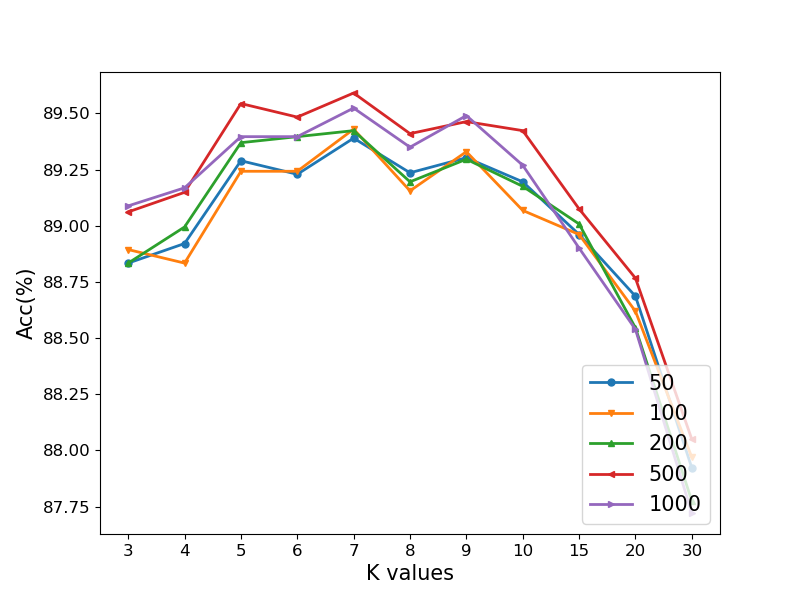
\includegraphics[width=1.0\linewidth]{img/LSML.png}
        \caption{Accuracy of LSML metric learning}
        \label{fig:lsml}
    \end{minipage}
    \begin{minipage}[t]{0.48\linewidth}
        \centering
        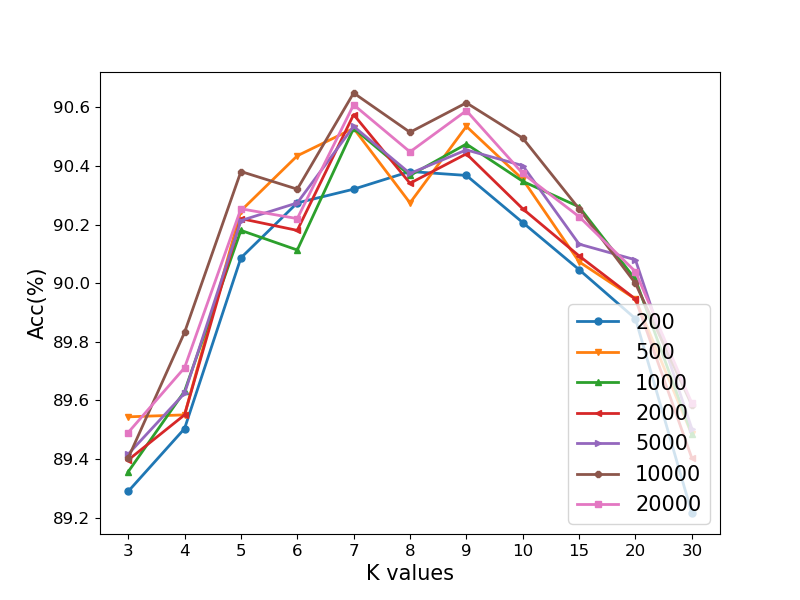
\includegraphics[width=1.0\linewidth]{img/LSML-PCA.png}
        \caption{Accuracy of LSML after PCA}
        \label{fig:lsml-pca}
    \end{minipage}
\end{figure}



Inspired by the experiment results for ITML, we continue to try applying LSML to PCA-reduced dataset. The result is listed in Table \ref{tab:lsml2}. 

Although the improvement after dimensionality reduction is not very significant in accuracy, we may still conclude that PCA is a useful pre-processing technique for weakly supervised metric learning because it enables us to sample more data-points, thus gaining better learned metrics for the KNN classification task. Therefore, for later experiments, we will train the learned metrics after performing PCA on the original data-set.


\subsubsection{SCML: Sparse Compositional Metric Learning}

We first reduce the dimension of the original data-set to 64-dimensions. Then we use SCML to learn the metric and evaluate the KNN classification accuracy. The triplets are sampled by taking 3 neighbours of the same class and 10 neighbours from different classes for each point and then runs the SCML algorithm on these triplets.

The experiment result is shown in Table \ref{tab:scml}. It can be found that SCML does not reach an outstanding performance on our data-set even after PCA.

\begin{table}[h]
\centering
\caption{KNN Accuracy of SCML on PCA-reduced data-set \label{tab:scml}}
\begin{tabular}{cc}
\hline
K   & Accuracy \\ \hline
3   & 86.295\% \\
4   & 86.643\% \\
5   & 87.327\% \\
6   & 87.494\% \\
7   & 87.849\% \\
8   & 87.675\% \\
9   & 87.796\% \\
10  & 87.782\% \\
15  & \textbf{87.956\%} \\
20  & 87.541\% \\
30  & 87.112\% \\ \hline
Avg & 87.406\% \\ \hline
\end{tabular}
\end{table}


\subsubsection{RCA: Relative Components Analysis}

We explore the effect of RCA metric learning by changing our sampling strategy on the PCA-reduced data-set. The experiment result can be found in Table \ref{tab:rca}. Generally speaking, the larger the sampling size, the better the learned metrics. 

\begin{table}[h]
\centering
\caption{KNN Accuracy of RCA on PCA-reduced data-set with different $\mathtt{num\_chunks}\times\mathtt{chunk\_size}$\label{tab:rca}}
\begin{tabular}{cccccccc}
\hline
K   & 100×2             & 100×8             & 100×32            & 200×32            & 500×32            & 500×40            \\ \hline
3   & 84.667\%          & 89.376\%          & 89.705\%          & 89.678\%          & 89.611\%          & 89.624\%          \\
4   & 85.022\%          & 89.329\%          & 89.685\%          & 89.698\%          & 89.685\%          & 89.658\%          \\
5   & \textbf{85.686\%} & 89.765\%          & 90.247\%          & 90.214\%          & 90.167\%          & 90.281\%          \\
6   & 85.659\%          & 89.778\%          & 90.100\%          & 90.207\%          & 90.194\%          & 90.247\%          \\
7   & 85.719\%          & 90.227\%          & 90.354\%          & 90.395\%          & \textbf{90.395\%} & 90.475\%          \\
8   & 85.692\%          & 90.100\%          & 90.294\%          & 90.281\%          & 90.307\%          & 90.448\%          \\
9   & 85.833\%          & 90.234\%          & 90.240\%          & \textbf{90.515\%} & 90.334\%          & 90.395\%          \\
10  & 85.759\%          & \textbf{90.240\%} & \textbf{90.368\%} & 90.455\%          & 90.314\%          & \textbf{90.488\%} \\
15  & 85.645\%          & 89.939\%          & 90.080\%          & 90.361\%          & 90.301\%          & 90.294\%          \\
20  & 85.284\%          & 89.772\%          & 89.879\%          & 90.187\%          & 90.013\%          & 90.080\%          \\
30  & 84.647\%          & 89.350\%          & 89.524\%          & 89.812\%          & 89.604\%          & 89.658\%          \\ \hline
Avg & 85.419\%          & 89.828\%          & 90.043\%          & \textbf{90.164\%} & 90.084\%          & 90.150\%          \\ \hline
\end{tabular}
\end{table}
